\documentclass[conference]{IEEEtran}
\IEEEoverridecommandlockouts
\usepackage{graphicx}
\usepackage{amsmath}

\title{Implementation and Evaluation of a Chord-Based Distributed Hash Table}
\author{
  \IEEEauthorblockN{Carlo Alberto Cacopardo}
  \IEEEauthorblockA{UiT The Arctic University of Norway} \\
  \IEEEauthorblockN{Ruben Sebastian Rogne}
  \IEEEauthorblockA{UiT The Arctic University of Norway}
}

\begin{document}
\maketitle

\begin{abstract}
We implemented a Chord based distributed hash table (DHT) with an HTTP API and evaluated it on the IFI cluster with up to 16 nodes. Experiments were automated end-to-end, measuring the time for 1000 operations and the average latency per operation. Results show correct routing and a steady increase in operation time as the ring grows, consistent with Chord’s $O(\log n)$ lookup property. However, measurements also reveal a significant constant per hop overhead from Python and HTTP. We discuss strengths, limitations, and the most impactful directions for improvement.
\end{abstract}

\section{Introduction}
Chord maps nodes and keys onto a ring using consistent hashing and routes via finger tables~\cite{stoica2003chord}. Each node maintains pointers to its predecessor, successor, and $O(\log n)$ fingers, enabling lookups in $O(\log n)$ hops while storing only $O(\log n)$ state.  
We implemented a static membership verson of Chord with a (\texttt{PUT}/\texttt{GET}) API and evaluated its performance on the IFI cluster under different scales.

\section{Design and Implementation}
\subsection{Identifiers and Responsibility}
Node addresses (\texttt{host:port}) and keys are hashed with SHA-1 into a $2^{160}$ identifier space. A node is responsible for keys in the interval $(\text{predecessor}, \text{self}]$. Any node can decide locally whether to serve or forward a request.

\subsection{Routing}
Lookups use the closest preceding finger. Forwarded requests include a TTL header (default 32) to guard against routing loops, though no loops occurred in testing.

\subsection{Finger Tables}
At startup, nodes read a shared \texttt{peers.json} to build $\lceil \log_2 n \rceil + 1$ fingers with starting points $id + 2^i \bmod 2^{160}$. After initialization, nodes discard the global view and keep only local state (predecessor, successor, fingers), adhering to Chord’s principle that the system is not fully connected.

\subsection{HTTP API}
The server exposes:  
\texttt{GET /storage/<key>} (returns value or 404),  
\texttt{PUT /storage/<key>} (stores value),  
\texttt{GET /network} (neighbors and fingers in JSON),  
\texttt{GET /helloworld} (returns \texttt{host:port} for sanity checks).  

Values are stored in memory only. The server is multi threaded (per connection) and terminates after 15 minutes to avoid stragglers on the shared cluster.

\subsection{Automation and Methodology}
\textbf{\texttt{run.sh}.} Automates the full lifecycle: kill stale servers, launch $N$ nodes, generate \texttt{peers.json}, wait for sockets, run correctness tests, benchmark, and clean up. This eliminates human error (wrong ports, leftover processes) and ensures reproducibility.

\textbf{\texttt{bench.py}.} Generates random key–value pairs, executes a fixed number of \texttt{PUT}s and \texttt{GET}s against random entry nodes, and logs results to CSV. Randomization spreads the load and highlights routing costs.

\section{Evaluation}
We tested configurations of 1, 2, 4, 8, and 16 nodes. Each was run 5 times with \texttt{./run.sh N --bench}. Aggregate times for 1000 operations: 1 node 0.636\,s (1575 ops/s), 2 nodes 1.291\,s (787 ops/s), 4 nodes 3.219\,s (321 ops/s), 8 nodes 6.617\,s (152 ops/s), 16 nodes 14.580\,s (68 ops/s).

\begin{figure}[t]
  \centering
  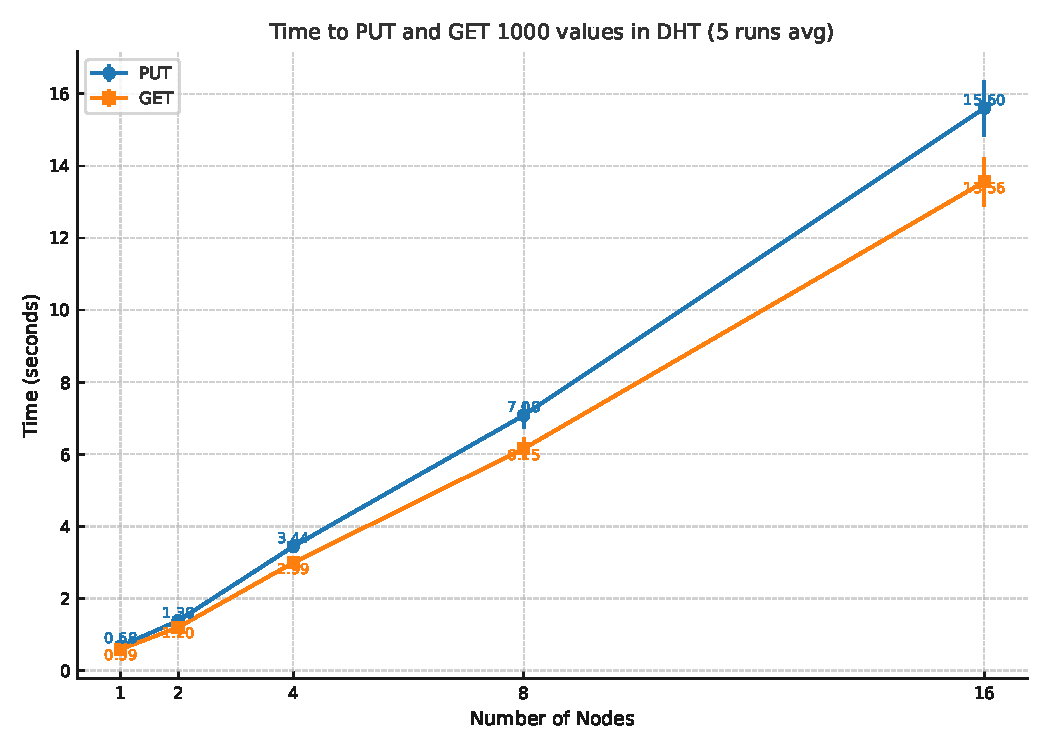
\includegraphics[width=0.95\columnwidth]{throughput.pdf}
  \caption{Execution time for 1000 \texttt{PUT} and 1000 \texttt{GET} operations across 1 to 16 nodes (5 runs avg; error bars show std.\ dev.).}
  \label{fig:time}
\end{figure}

\begin{figure}[t]
  \centering
  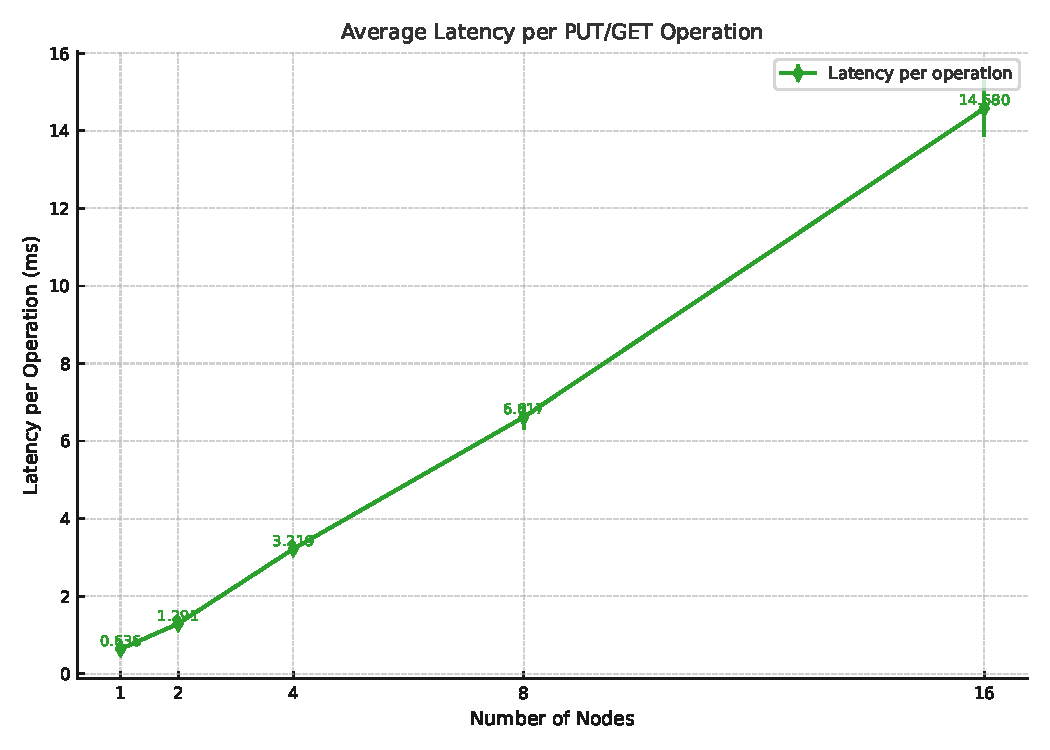
\includegraphics[width=0.95\columnwidth]{latency.pdf}
  \caption{Average latency per operation (ms/op) across network sizes (5 runs avg; error bars show std.\ dev.).}
  \label{fig:latency}
\end{figure}

\subsection{Findings}
\textbf{Correctness.} Keys stored on any node could be retrieved from any node; nonexistent keys returned 404. Requests consistently reached the responsible node.  

\textbf{Scaling.} Operation times increased with network size (Fig.~\ref{fig:time}). Latency grew from $\approx$0.64\,ms (1 node) to $\approx$14.6\,ms (16 nodes), consistent with $O(\log n)$ growth. However, absolute costs were dominated by constant hop overhead: Python request handling, HTTP parsing, thread scheduling, and TCP setup.  

\textbf{Stability.} Narrow error bars indicate steady cluster conditions. Performance is CPU/overhead bound rather than dominated by random network jitter.

\section{Strengths and Limitations}
\subsection{What Worked}
\begin{itemize}
  \item Local responsibility checks were simple and reliable.
  \item Closest preceding finger routing converged quickly.
  \item The TTL header was an effective safeguard against loops.
  \item Full automation (\texttt{run.sh} $\rightarrow$ testers $\rightarrow$ bench) was critical for obtaining clean, reproducible results.
\end{itemize}

\subsection{Weaknesses}
Although the system works as intended for small experiments, several clear weaknesses became evident during testing. The first and most visible issue is the drop in throughput as more nodes are added. With only one node the system could process over 1500 operations per second, but with sixteen nodes this fell to fewer than 70. 
In theory, Chord lookups should grow only logarithmically with the number of nodes, which is a very gentle curve. What we observed instead was a much steeper slowdown. 
The reason is not the Chord algorithm itself, but the constant overhead of our chosen implementation. Every hop in the path adds the cost of setting up a TCP connection, parsing an HTTP request, and spawning a new Python thread. These fixed costs accumulate quickly, so the scaling curve ends up being dominated by engineering overhead rather than the theoretical efficiency of the protocol.

A second limitation is the lack of churn handling. Our system assumes that the network membership is fixed once it starts up. If a node crashes or a new node wants to join, the ring cannot adapt. In real distributed systems, churn is the norm rather than the exception: machines fail, processes are restarted, and resources appear or disappear. Without stabilization routines to repair finger tables and update successor pointers, the ring will eventually break, leaving some keys unreachable. 

Closely related to this is the absence of replication. Each key is stored on exactly one node, and if that node goes down the data is lost permanently. The original Chord design recommends keeping replicas on a few successors to guard against such failures. We skipped this feature in order to keep the code simple, but it means our system cannot tolerate faults. For any real use case, this is a serious issue.

Finally, our benchmarking setup used only a single client sending requests one after another. This is good enough to measure baseline latency, but it does not reflect how distributed systems are actually used. In reality, many clients would interact with the system at the same time, creating load spikes, delays, and lock contention inside each server. Without testing concurrency, we cannot know how well the system would hold up under pressure. 

It is very likely that tail latencies would increase significantly and hidden bottlenecks would appear.

To sum up, the prototype demonstrates that the core routing logic of Chord works correctly, but it is limited by its environment. The heavy cost of Python and HTTP, the lack of churn support, the absence of replication, and the simplified benchmarking setup all combine to show that while the system is educational and functional, it is far from being production ready.


\section{Future Improvements}
\textbf{Transport.}  
The current prototype relies on Python builtin HTTP server, which opens a new TCP connection for every forwarded request. This makes each hop expensive and explains why throughput falls so sharply when more nodes are added. A concrete improvement would be to reuse TCP connections through HTTP keep alive or to switch the RPC layer to something lighter with persistent sockets. 

\textbf{Latency aware routing.}  
At present, fingers are chosen purely by identifier distance when we build the \texttt{peers.json} file. This is simple but ignores the real network delays between IFI cluster nodes. Dabek et al.\ showed that incorporating proximity measurements when selecting fingers reduces lookup time significantly~\cite{dabek2004dht}. In our case, extending the startup phase to measure round trip times and prefer low latency neighbors could reduce the absolute slope of Fig.~\ref{fig:latency}, even if the overall growth remains logarithmic.  

\textbf{Adaptive stabilization.}  
Our implementation uses a one shot initialization: once the ring is built from \texttt{peers.json}, it never changes. This makes the system brittle under churn. Adding a simple periodic stabilization task in Python would allow nodes to repair broken links if a peer fails. Tauber et al.\ demonstrate that adapting stabilization intervals to network conditions can keep lookup consistency high while reducing overhead~\cite{tauber2010autonomic}.  

\textbf{Robustness.}  
Currently, keys are stored in memory only and only on the responsible node. This makes failures catastrophic: if a process dies, its entire key range is lost. A practical next step would be to store values redundantly on each node successors, which would require only minor changes to the \texttt{PUT} handler. Replication would not fix the performance bottleneck, but it would make the system solid enough for longer experiments.  

\textbf{Concurrency.}  
The benchmark client executes requests sequentially, which hides many real bottleneks. Extending \texttt{bench.py} to spawn several concurrent clients would allow us to measure how the servers behave under load. This would stress test the threaded HTTP handler, reveal lock contention on the storage dictionary, and provide a more realistic picture of tail latency and throughput under multi client use.  


\section{Conclusion}
We implemented a Chord based DHT that meets the assignment API requirements, routes correctly, and runs across 1 to 16 nodes. Measurements confirmed the expected $O(\log n)$ lookup behavior but highlighted the heavy overhead of a Python/HTTP implementation. Automation scripts ensured reproducibility and clean comparisons. This work provides a solid baseline for extending the system with churn handling, replication, and lower overhead transports.

\bibliographystyle{IEEEtran}
\bibliography{IEEERef}

\end{document}
